\documentclass[a5paper]{article}
\usepackage[a5paper, top=8mm, bottom=8mm, left=8mm, right=8mm]{geometry}

\usepackage{polyglossia}
\setdefaultlanguage[babelshorthands=true]{russian}

\usepackage{fontspec}
\setmainfont{FreeSerif}
\newfontfamily{\russianfonttt}[Scale=0.7]{DejaVuSansMono}

\usepackage[font=scriptsize]{caption}

\usepackage{amsmath}
\usepackage{amssymb,amsfonts,textcomp}
\usepackage{color}
\usepackage{array}
\usepackage{hhline}
\usepackage{cite}
\usepackage{textcomp}

\usepackage[hang,multiple]{footmisc}
\renewcommand{\footnotelayout}{\raggedright}

\PassOptionsToPackage{hyphens}{url}\usepackage[xetex,linktocpage=true,plainpages=false,pdfpagelabels=false]{hyperref}
\hypersetup{colorlinks=true, linkcolor=blue, citecolor=blue, filecolor=blue, urlcolor=blue, pdftitle=1, pdfauthor=, pdfsubject=, pdfkeywords=}

\newlength\Colsep
\setlength\Colsep{10pt}

\usepackage{tabu}

\usepackage{graphicx}
\usepackage{indentfirst}
\usepackage{multirow}
\usepackage{subfig}
\usepackage{footnote}
\usepackage{minted}

\newcommand{\todo}[1] {
\begin{center}\textcolor{red}{TODO: #1}\end{center}
}

\newcommand{\attribution}[1] {
	\vspace{-5mm}\begin{flushright}\begin{scriptsize}%\textcolor{gray}
	{\textcopyright\, #1}\end{scriptsize}\end{flushright}
}

\sloppy
\pagestyle{plain}

\title{Лекция 3: Моделирование, UML}
\author{Юрий Литвинов\\\small{yurii.litvinov@gmail.com}}
\date{}

\begin{document}

\maketitle
\thispagestyle{empty}

\section{Моделирование}

Эта лекция начнёт рассказ о моделировании --- важном инструменте для создания и, главное, описания архитектуры системы. Труд архитектора обычно находит внешнее выражение в архитектурной документации, ключевой составляющей которой являются визуальные модели программного обеспечения. Для создания визуальных моделей существует много визуальных языков, формальных и не очень, мы в этом курсе рассмотрим UML, с отвлечениями на некоторые другие визуальные языки.

Но начать следует с понятия ``модель''. \textit{Модель} --- это упрощённое подобие некоторого объекта или явления, нужное для изучения некоторых его свойств, абстрагируясь от сложности того, что они моделируют. Модели используются повсюду --- математические модели, реальные модели (например, модели самолётов для изучения их аэродинамических характеристик) и, конечно, модели в разработке программного обеспечения.

Модели принципиально содержат меньше информации, чем реальность. Нет смысла максимально точно моделировать какой-то объект, ведь если сложность не проблема, можно изучать и сам объект. А раз так, то каждая модель всегда создаётся для какой-то определённой цели, выделяя из моделируемого объекта или явления только те свойства, которые важны для исследования. В частности, поэтому при моделировании ПО рисовать диаграммы ``вообще'' в корне неправильно. Кроме того, модели субъективны. В случае с ПО архитектор сам решает, что следует показать на модели, а что нет. Это, в частности, нужно опять-таки для того, чтобы отделять существенные свойства от несущественных. И наконец, модели всегда ограничены --- они в принципе не могут моделировать бесконечную сложность физических явлений или мельчайшие подробности программного кода. Так что стремиться к полноте при моделировании не только бессмысленно, но и просто нельзя, иначе модели станут бесполезны.

Кстати, есть хорошее высказывание про моделирование, более чем применимое к миру разработки ПО: ``All models are wrong, some are useful''. Именно так, модели всегда неправильны (по вышеизложенным соображениям, они не могут содержать всю информацию о системе), но некоторые из них полезны. Поэтому моделирование часто не применяется при разработке ПО вовсе (потому что зачем, они всё равно врут, а создать и поддерживать модель --- это большая работа). Поэтому, возможно, часть этого курса про моделирование конкретно вам никогда в жизни не пригодится. Но если всё-таки в вашей компании вдруг решат использовать визуальные модели, вы должны знать, что это, зачем и как это делать. И главное, чего ожидать --- не точности и полноты, а именно полезности.

\subsection{Модели в проектировании ПО}

Полезность моделей при проектировании ПО заключается прежде всего в управлении сложностью. В предыдущей лекции говорилось, что сложность --- это неотъемлемое свойство программного обеспечения, так что модели ПО, в отличие от математических или физических моделей, сами бывают довольно сложны. Но возможность взглянуть на систему с нескольких разных точек зрения, выделяя каждый раз разные существенные моменты, оказывается очень ценной при проектировании и документировании системы. На самом деле, модели ПО часто моделируют не только само ПО, но и окружение, в котором оно работает --- будь то автоматизируемый бизнес-процесс или внешние системы или пользователи.

Вот небольшой пример модели из аналогичного курса универитета Южной Калифорнии (на него мы далее тут будем неоднократно ссылаться с любезного согласия автора курса проф. N. Medvidovic):

\begin{center}
	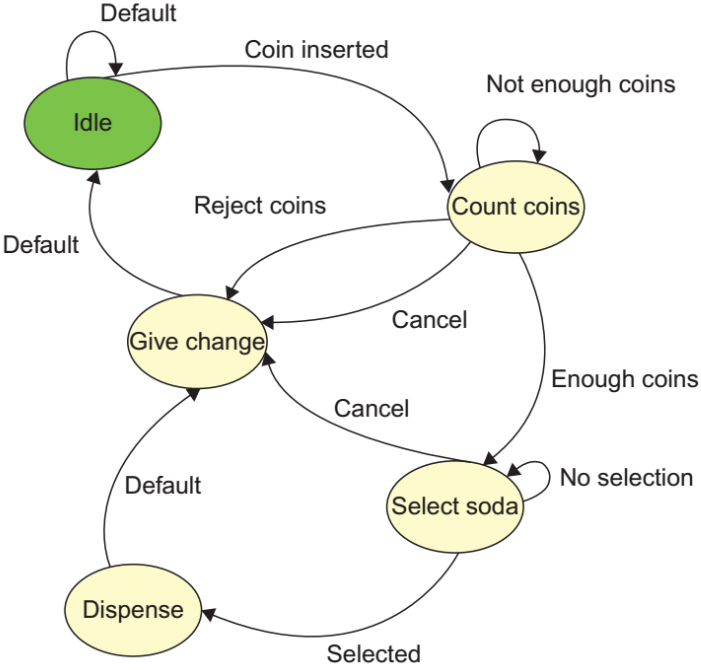
\includegraphics[width=0.5\textwidth]{vendingMachine.png}
\end{center}

Видно, что модель ПО может быть довольно неформальна (хотя на самом деле это конечный автомат, пожалуй, одна из самых формальных моделей), проста (хотя за каждым состоянием и переходом может скрываться очень много строк кода), и при этом полезна. Причём не только с иллюстративной, но и с прагматической точки зрения --- можно отследить множество достижимых состояний, проверить, что автомат всегда может вернуться в исходное состояние. Это ценное свойство всех моделей ПО --- они позволяют (в большей или меньшей степени, в зависимости от используемого формализма) понять, проанализировать и даже протестировать систему ещё до того, как будет написана первая строчка кода.

Используемые нотации и способы моделирования бывают разные и зависят от целей моделирования:

\begin{center}
	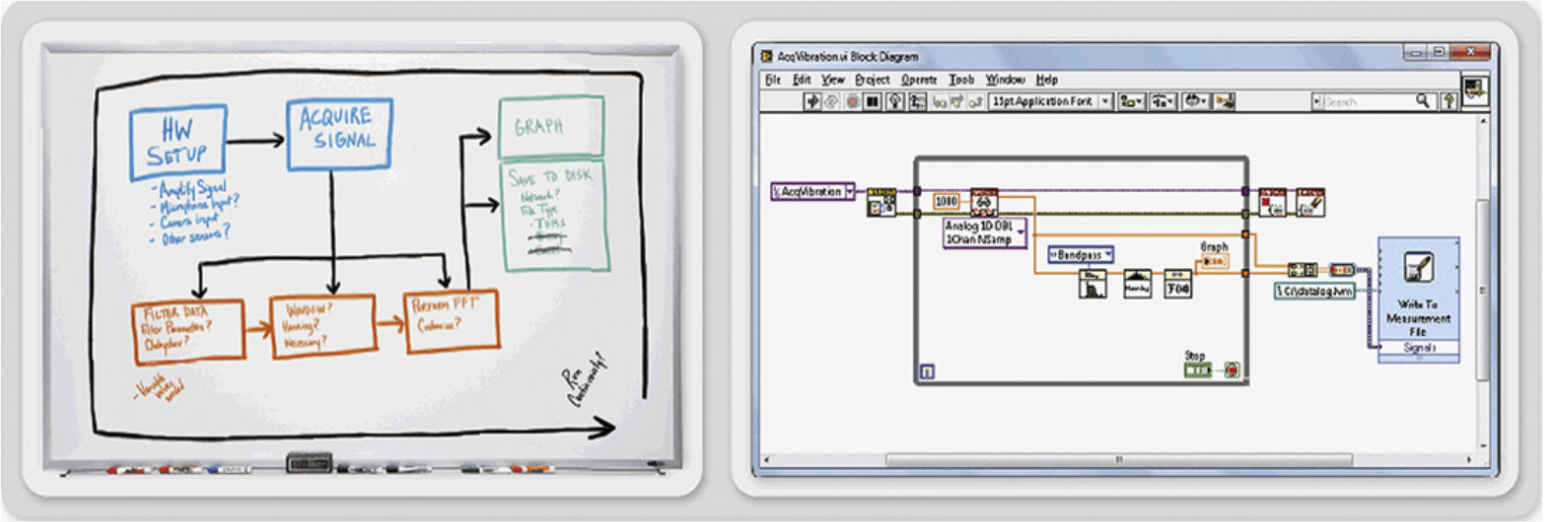
\includegraphics[width=0.9\textwidth]{sketchesVsFormalNotations.png}
	\attribution{N. Medvidovic}
\end{center}

Самые ходовые модели, на самом деле, неформальные. Большая часть полезных моделей служит только для поддержки общения, такие модели рисуются на доске, их обсуждают и тут же стирают, в лучшем случае фотографируя. Более формальные модели используются в документации, там их некому вживую пояснить, поэтому требуется использовать более-менее стандартные языки моделирования (например, UML) --- чтобы даже если систему отдали на аутсорсинг в Индию, архитектуру поняли бы однозначно. Самые формальные модели --- исполнимые, это полноценные языки программирования, только в графическом синтаксисе (например, LabVIEW, модель на картинке, справа --- на нём по-настоящему программируются микроконтроллеры и даже целые их сети).

\subsection{Архитектурные модели}

Как говорилось в первой лекции, архитектура --- это набор основных решений, принятых для данной системы. \textit{Архитектурная модель} --- это некоторый артефакт, который отражает некоторые или все эти решения. Описание архитектуры может иллюстрироваться сразу многими архитектурными моделями, каждая из которых описывает свой набор важных решений. Какое из решений считать важным, решает архитектор.

Архитектурное моделирование --- это процесс уточнения и документирования архитектурных решений. Модели делают решения явными и часто сами ``задают вопросы'' архитектору, позволяя лучше понять создаваемую архитектуру и заполнить пропущенные моменты. Лучше всего направляют архитектурную мысль языки, специально созданные для описания архитектуры (AADL, UML, IDEF, ...), так что правильный выбор нотации может быть критичен для успешности моделирования и разработки архитектуры вообще.

Однако существует опасность ``архитектурного паралича'' проекта, когда неопытная команда пытается настолько детально проработать архитектуру, что проект закрывается из-за нехватки денег ещё до того, как написана первая строчка кода. Чтобы этого избежать, надо определиться с тем,

\begin{itemize}
	\item какие архитектурные решения нуждаются в моделировании;
	\item на каком уровне детализации;
	\item насколько формально.
\end{itemize}

Естественно, самые важные части архитектуры должны получать больше всего внимания при моделировании. Под самыми важными следует понимать не те решения, которыми вы особо гордитесь, а то, что затронет большое количество пользователей или разработчиков системы. Не очень важным компонентам можно уделять меньше внимания --- описывать их менее подробно и/или менее формально. Помните, что моделирование выполняется не ради высшего блага, а чтобы упростить разработку, поэтому при выборе, что моделировать, важно учитывать соотношение трудозатрат и выгоды. Следует помнить также про процесс поддержки моделей --- при изменении архитектуры и кода диаграммы, возможно, тоже придётся перерисовывать, иначе они быстро потеряют всякий смысл. Стоимость создания и поддержания модели не должна быть больше преимуществ от её использования.

Немного подробнее о преимуществах, на которые можно надеяться при использовании моделирования. Модели --- это:

\begin{itemize}
	\item инструмент, направляющий и облегчающий проектирование --- особенно если используется подходящий визуальный язык, модели сами подсказывают направление архитектурной мысли и делают очевидными слабые места архитектуры;
	\item средство коммуникации между разработчиками --- ``one picture worth a thousand words'', с помощью диаграмм проще донести идею решения, диаграммы проще обсуждать, чем код или идеи, выраженные только словами;
	\item наглядный инструмент для общения с заказчиком --- бывают не очень формальные диаграммы, понятные неспециалистам. Проще (и выглядит более профессионально!) показать диаграммы, чем долго и утомительно рассказывать, что вы предлагаете;
	\item средство документирования и фиксации принятых решений --- в этом качестве диаграммы используются в архитектурных описаниях, использование стандартных визуальных языков повышает вероятность, что идеи будут правильно поняты коллегами, даже если вы не можете лично их передать;
	\item исходник для генерации кода --- бывают очень формальные диаграммы, по которым можно генерировать работающее приложение. Чаще, однако, так делать нет смысла, потому что между моделью и кодом есть так называемый \textit{семантический разрыв}, связанный с тем, что модель содержит принципиально меньше информации, чем надо для того, чтобы её можно было исполнить. Например, любой нормальный инструмент для рисования UML-диаграмм умеет генерировать заглушки классов (объявления классов и методов, даже с полями, но без реализаций), но это не то чтобы суперполезно, потому что сгенерированный код потом всё равно надо дописывать руками и поддерживать (и приводить к конкретно вашему стайлгайду). Так что в общем случае на возможность сгенерировать код по моделям лучше особо не рассчитывать.
\end{itemize}

\subsection{Виды моделей}

Рассмотрим, какого рода модели вообще используются при проектировании программного обеспечения.

\subsubsection{Естественный язык}

Самый распространённый вид моделей, который обычно даже моделями-то не считается --- это просто текст на естественном языке. Вот простой пример текстовой модели игры ``Посадка на луну'' из лекции проф. N. Medvidovic:

\begin{center}
	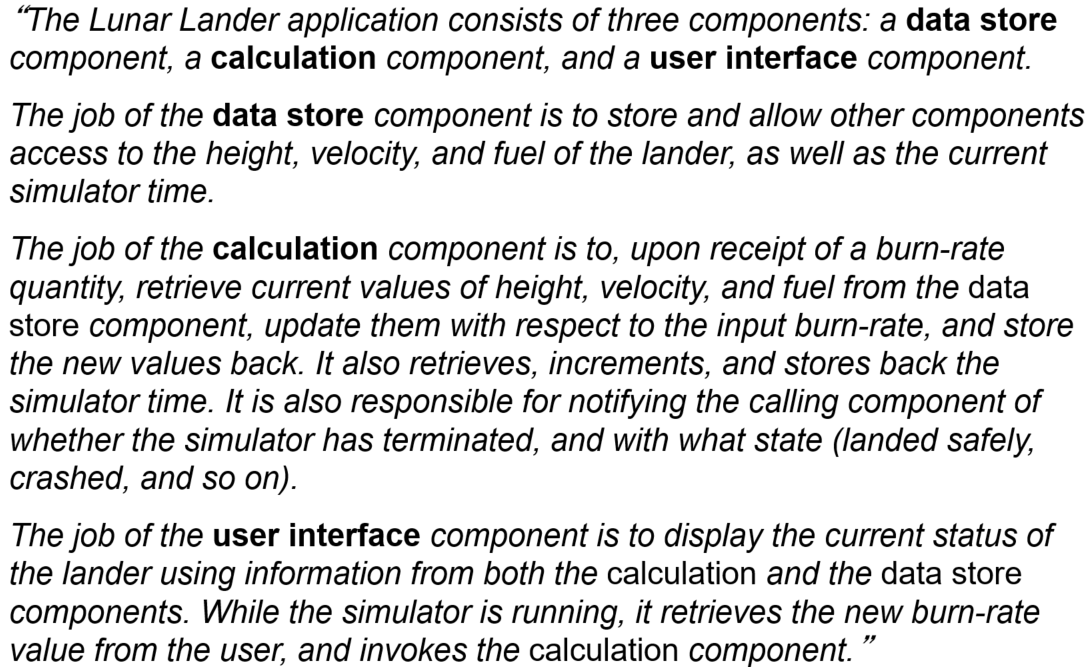
\includegraphics[width=0.6\textwidth]{naturalLanguage.png}
	\attribution{N. Medvidovic}
\end{center}

Преимущества моделей на естественном языке очевидны --- чтобы читать такие модели, не требуется учить синтаксис новых языков, язык очень выразителен (в буквальном смысле позволяет описать все мыслимые модели), максимально гибок. Недостатки, впрочем, тоже очевидны --- естественный язык неформален, не строг, слишком многословен, бесполезен для автоматической обработки (в этом плане последние достижения в NLP дают некоторую надежду, но пока что алгоритмы разбора текстов на естественных языках очень далеки от применения в инструментах разработки архитектуры).

\subsubsection{Неформальные графические модели}

Активно используются и неформальные графические модели --- диаграммы, рисуемые в PowerPoint, InkScape, Visio (без плагина UML) и подобных редакторах. На самом деле, такие диаграммы, скорее всего, встречаются в мире разработки ПО даже чаще, чем UML-диаграммы:

\begin{center}
	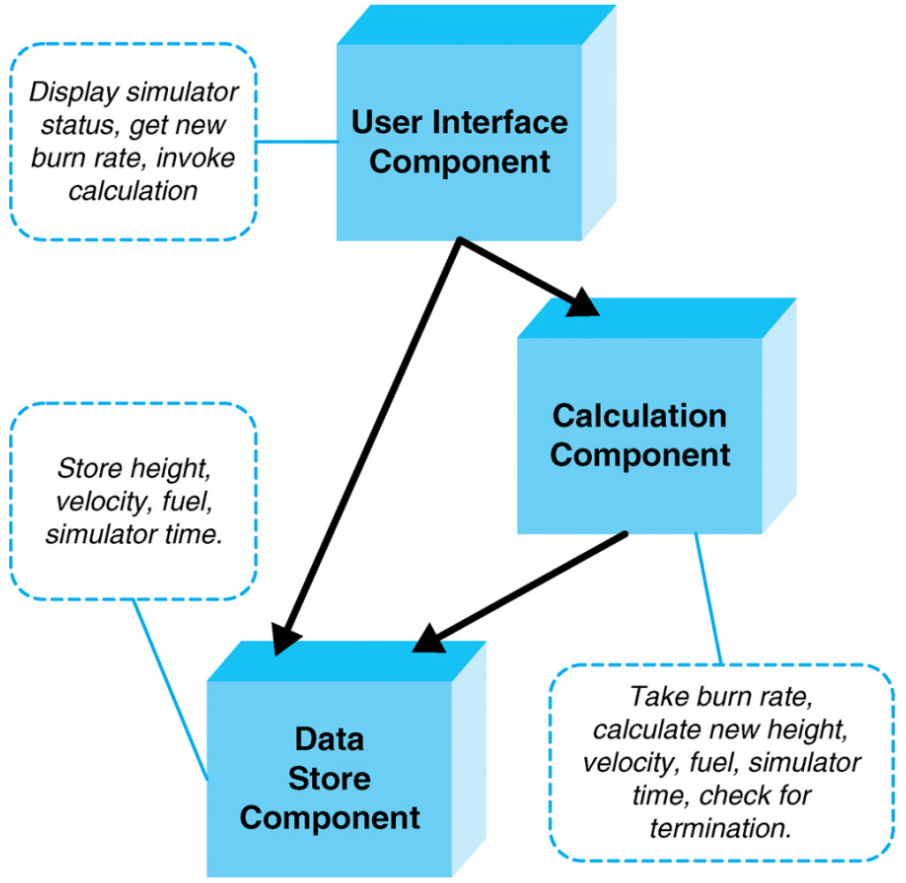
\includegraphics[width=0.4\textwidth]{informalModel.png}
	\attribution{N. Medvidovic}
\end{center}

Преимущества такого подхода --- простота понимания (опять-таки, не требуют специальных знаний), очень гибкая нотация, их можно сделать чисто внешне красивыми. Недостатки --- опять-таки неформальность, нестрогость и неоднозначность, и тут, в отличие от текстовых моделей, есть подводный камень --- неформальные диаграммы часто воспринимаются неспециалистами как формальные и строгие. Такие диаграммы всё ещё практически бесполезны для автоматической обработки. Фигуры и линии с их координатами обычно несложно достать из файлов сохранения, но потом их приходится мучительно парсить, чтобы программно понять смысл нарисованного. Например, в Visio фигура и текст, который внутри написан, могут быть формально никак не связаны и даже храниться в разных частях файла.

\subsubsection{Формальные графические модели}

Формальные графические модели --- это прежде всего модели на формальных языках типа UML, SysML, Entity-Relationship, IDEF0 и т.д., таких языков довольно много. Такие языки часто состоят из нескольких разных нотаций (или ``диаграмм''), позволяющих отдельно моделировать разные точки зрения на систему, стандартны --- в чём их главное преимущество перед способами, рассмотренными выше --- и, поэтому, имеют хорошую инструментальную поддержку (например, существует больше десятка только популярных UML-инструментов для создания архитектурных моделей, непопулярных тысячи). Важным достоинством является формальность языков, что может быть непривычно для людей, привыкших воспринимать UML как картинки --- у UML и у любого другого такого языка есть строгий синтаксис, описывающий множество корректных диаграмм, как и у текстовых языков программирования. Важный недостаток формальных графических моделей --- частое отсутствие строгой семантики (в UML из 14 видов диаграмм формальная семантика хоть как-то описана только для двух, хотя синтаксис подробно описан для каждой). Кроме того, поскольку такие языки поддерживают много точек зрения, между ними сложно обеспечить консистентность, сложно расширять языки и модифицировать их под свои нужды.

Вот пример трёх разных диаграмм (или ``подъязыков'') UML:

\begin{center}
	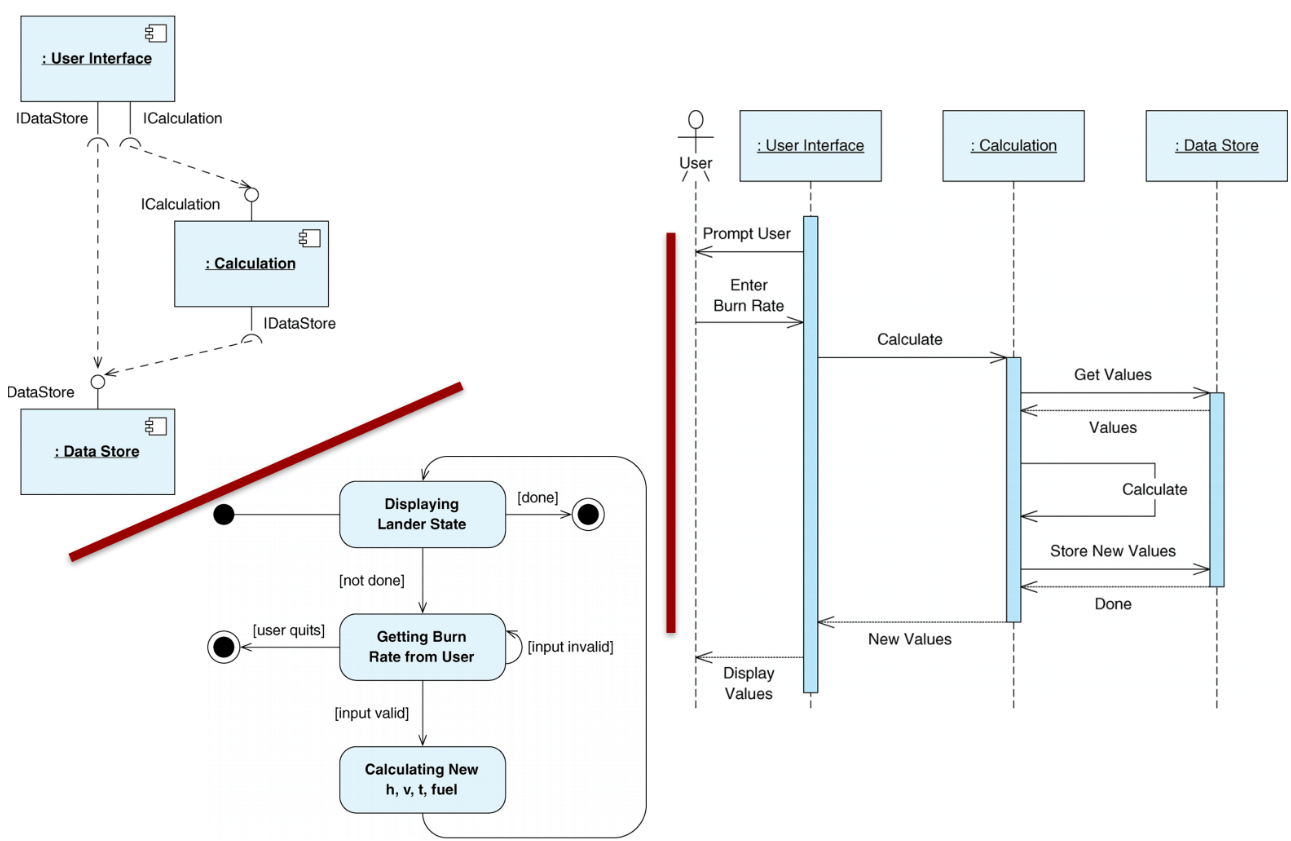
\includegraphics[width=\textwidth]{uml.png}
	\attribution{N. Medvidovic}
\end{center}

\subsubsection{Формальные текстовые языки}

Даже формальные графические языки недостаточно формальны (обычно не имеют исполнимой семантики, что ннеудивительно, потому что это языки моделирования всё-таки). Поэтому существуют и формальные текстовые языки описания архитектуры, например, AADL (может быть, VHDL можно отнести к таким языкам, хоть он слишком специфичен). Это языки, где компоненты системы и интерфейсы между компонентами описываются формально на языке программирования (но без реализации, конечно), выписываются и доказываются различные утверждения про моделируемую систему (например, ограничения на время отклика, пропускную способность). Пример описания архитектуры на AADL от проф. N. Medvidovic:

\begin{center}
	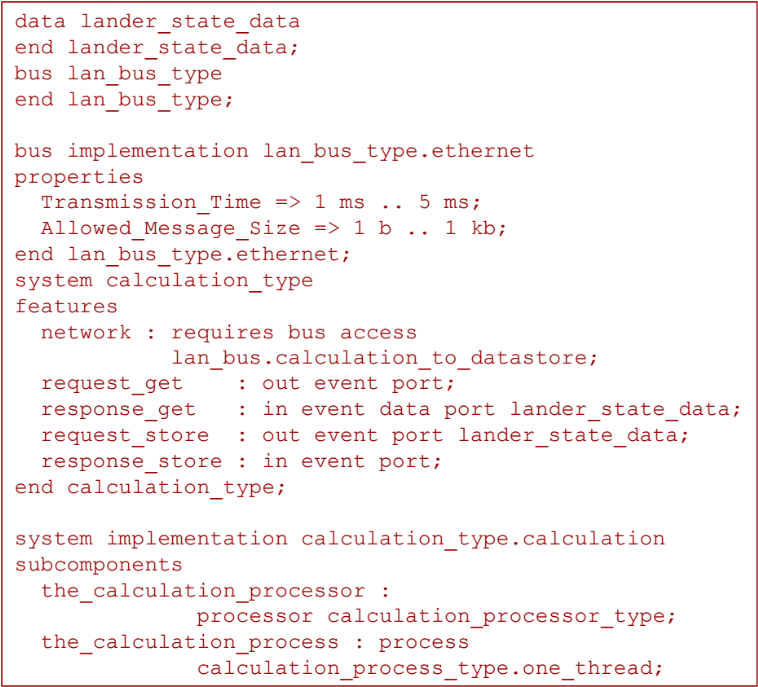
\includegraphics[width=0.65\textwidth]{aadl.png}
	\attribution{N. Medvidovic}
\end{center}

Используются такие языки в основном там, где требуется высокая надёжность и некоторые гарантии на параметры системы --- во встроенных системах, системах реального времени и т.д., они же используются часто при проектировании программно-аппаратных и аппаратных систем.

Основное преимущество подобного подхода --- возможность формального анализа свойств системы ещё до начала реализации, и для AADL существуют весьма продвинутые инструменты анализа. Основные недостатки --- слишком большая многословность и детальность (уже не нарисовать на доске), сложность в изучении и использовании (поэтому в результате одного опроса IT-компаний Турции выяснилось, что половина программистов слыхом не слыхивала про AADL).

\subsection{Ещё о визуальных моделях}

С архитектурными моделями связано ещё несколько понятий, которые мы пока подробно не рассматривали.

\begin{itemize}
	\item Метафора визуализации --- это договорённость о том, как будут представляться сущности языка. Например, в UML классы представляются в виде прямоугольников, разделённых на три области (имя класса, поля и методы), а в нотации Буча классы представлялись в виде облаков, нарисованных пунктирными линиями (а объекты --- в виде облаков, нарисованных сплошными линиями; ну а что, классы --- это что-то абстрактное). Поскольку программное обеспечение незримо, метаформа визуализации --- не более чем договорённость между программистами.
	\item Точка зрения моделирования --- какой аспект системы и для кого моделируется. Наличие такого понятия связано с тем, что модель принципиально проще моделируемой системы, так что приходится выбирать, какие детали оставить за её рамками. Бывают модели для программистов, по которым они должны понять, какие классы и с какими методами надо реализовать, бывают --- для менеджеров, чтобы те могли видеть, сколько уже реализовано и сколько ещё осталось, бывают --- для заказчиков, чтобы объяснить им, что в итоге получится и почему столько стоит. Перед тем, как рисовать диаграмму, важно понять, для кого и зачем мы её рисуем. Не следует рисовать диаграммы просто потому что мы можем.
	\item Семантический разрыв --- принципиальная неспособность модели полностью специфицировать систему; разрыв между информацией, содержащейся в модели и информацией, необходимой, чтобы компьютер мог выполнить программу, которую эта модель описывает. Впрочем, семантический разрыв --- это не приговор, исполнимые модели бывают и активно используются (впрочем, если быть точными, исполнимая модель --- это не модель, а программа на графическом языке). Чаще всего, однако, в реальной жизни встречаются одноразовые модели --- нужные только для того, чтобы передать идею. Их не то что нельзя исполнить, их часто нельзя даже понять без помощи автора.
\end{itemize}

\section{UML}

Unified Modeling Language (UML) --- пожалуй, самый популярный визуальный язык, используемый для разработки программного обеспечения, стандарт де-факто архитектурного моделирования. Пользуются им далеко не все проекты и компании, но знать его должен каждый уважающий себя программист и, тем более, архитектор, поэтому придётся потерпеть довольно нудный рассказ про UML далее. 

UML не любят, в частности, из-за его сложности --- на самом деле это не один язык, а порядка 14 разных языков, объединённых единым стандартом и единым описанием синтаксиса (то есть метамоделью). Обычно когда говорят UML, имеют в виду диаграммы классов, но это только один из 14 языков, бывают совсем другие нотации, описывающие систему с разных точек зрения.

UML разрабатывается консорциумом Object Management Group (OMG), в который входят крупные IT-компании и университеты (более сотни). OMG же стоит за такими стандатрами, как CORBA и BPMN. Некоторые версии UML (1.4.2 и 2.4.1, не очень свежие, но good enough) приняты как международные стандарты ISO. Первая из получивших распространение стандартизованная версия UML имела номер сразу 1.1 и появилась в 1997 году, до неё была спецификация 0.9 (1996 год), обратите внимание, примерно в то же время, когда появились первые версии Java. 

Появился UML не из воздуха: компания Rational наняла трёх ведущих методологов, занимавшихся визуальными языками и, собственно, методологией разработки ПО --- Айвара Якобсона, Джеймса Рамбо и Гради Буча (того самого Гради Буча, картинки из знаменитой книжки которого ``Object-oriented analysis and design'' были в предыдущей лекции). Каждый и этих уважаемых людей уже имел свою, и популярную, методологию проектирования. Буч был автором ``метода Буча'' и, кстати, сооснователем компании Rational, Рамбо был автором Object Modeling Technique (откуда в UML пришли диаграммы классов по сути), Якобсон --- автор Object-oriented software engineering, откуда в UML пришли диаграммы случаев использования. Была создана не только единая нотация, призванная покончить с языковой разрозненностью в области архитектуры в начале 90-х, но и единая методология разработки ПО: Rational Unified Process (RUP), бывшая популярной в конце девяностых, но побеждённая Agile-методологиями в начале двухтысячных. RUP предполагал активное использование UML, естественно. И так уж получилось, что компания Rational была первой на рынке с инструментами поддержки UML и RUP (кто бы мог подумать), стала фактическим монополистом в конце 90-х и, наверное, неплохо на этом заработала.

Дальнейшее развитие UML имеет одну серьёзную веху --- UML 2.0 (2005 год), когда язык существенно переработали и приспособили не только для разработки программного обеспечения, но и для аппаратных систем тоже (используется он до сих пор всё-таки в основном программистами, у инженеров и так всё хорошо было с визуальными нотациями и их инструментальной поддержкой). Нотация языка тоже существенно поменялась (например, диаграммы активностей и диаграммы конечных автоматов сделали двумя отдельными языками), так что это иногда приводит к путанице --- в интернетах полно диаграмм в старой нотации. Актуальная на данный момент версия UML --- 2.5.1, принятая в декабре 2017 года.

В UML определён механизм стандартных расширений, даже целых два --- \textit{профили} и \textit{метамоделирование}. Профили --- механизм легковесного расширения, позволяют уточнить уже существующую нотацию UML для использования в какой-то конкретной предметной области. Метамоделирование позволяет взять стандарт UML и его подредактировать, добавив новые элементы или убрав существующие. Это гораздо более трудоёмко, чем профили, и не все инструменты поддерживают такой подход, тогда как профили более-менее широко поддержаны. Тем не менее, и профили, и метамоделирование активно используются самим консорциумом OMG, так что у UML появились языки-``родственники'' (например, SysML), которые по сути расширения UML через метамоделирование. Есть и куча стандартных профилей UML, но мы не будем в этом курсе на них останавливаться.

\subsection{История UML}

Вот замечательный рисунок из \url{https://modeling-languages.com/history-modeling-languages-one-picture-j-p-tolvanen/}, показывающий взаимосвязь между разными визуальными языками:

\begin{center}
	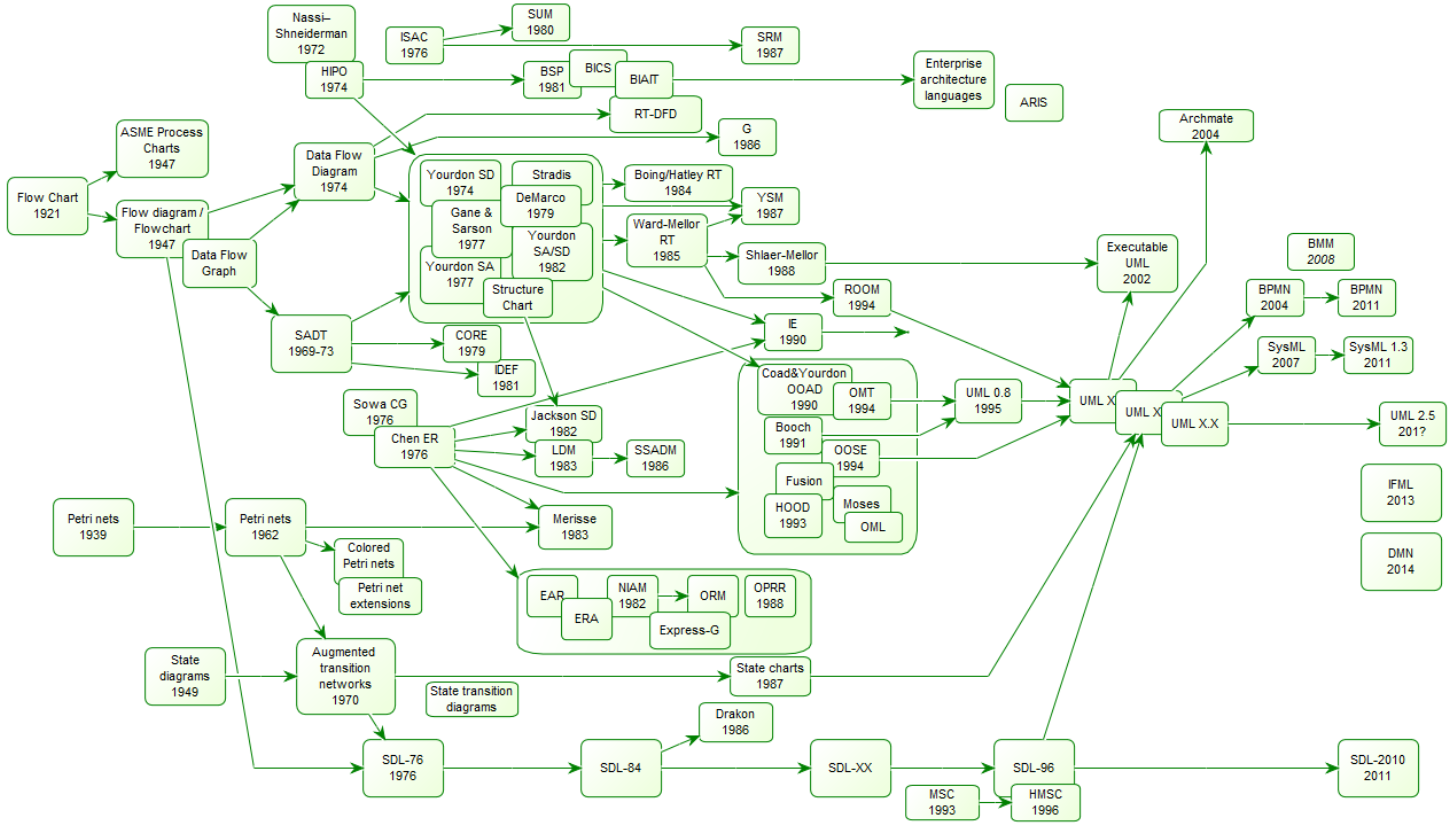
\includegraphics[width=\textwidth]{umlHistory.png}
\end{center}

Как видно из картинки, всё началось ещё до появления электронных компьютеров, различного рода диаграммы использовались давным-давно. Однако серьёзная потребность в моделировании при разработке ПО возникла только в конце 60-х годов, когда уже появились высокоуровневые языки программирования и программы начали становиться сложнее рассчётов по формуле. В это время появляются нотации, коnорые живы до сих пор: Data Flow Diagram, SADT (Structured Analysis and Design Technique), диаграммы Насси-Шнейдермана (из которых потом появился довольно известный нынче язык Scratch). На конец 1970-х приходится первый активный всплеск интереса к визуальным языкам и методологиям, появляются нотации SDL (Specification and Description Language), Entity-Relationship, IDEF, все они более чем живы до сих пор (SDL стандарт де-факто при описании телекоммуникационных протоколов, ER --- при проектировании баз данных, емейство языков IDEF применяется в анализе бизнес-процессов). 

Второй пик развития приходится на конец 80-х --- начало 90-х (поиски серебряной пули и языков 4-го поколения, которые повысили бы продуктивность труда программиста так же, как в своё время языки высокого уровня повысили продуктивность по сравнению с ассемблером). Каждая уважающая себя IT-компания считала своим долгом создать свою уникальную технологию на основе визуальных языков, получить огромный прирост производительности (в этом никто особо не преуспел) и ни с кем не поделиться секретом. Тут появляются языки, которые потом лягут в основу UML (нотация Буча, OOSE, OMT), языки, которые войдут в UML как часть, но продолжат развиваться независимо --- SDL, State charts (диаграммы конечных автоматов --- казалось бы, общеизвестная вещь, но формализованы они были Харелом только в 1987 году). Почётного упоминания заслуживает ДРАКОН (Дружественный Русский Алгоритмический язык, Который Обеспечивает Наглядность) Паронджанова, язык G, который до сих пор используется в LabVIEW и средах на её основе --- Robolab и, внезапно, стандартной среде для программирования роботов Lego. Андрей Николаевич Терехов создавал редакторы SDL и технологию RTST примерно в это же время.

В 1995 году появляются первые нестандартизованные спецификации UML, которые оканчивают эпоху языкового зоопарка, дальше UML плавно развивается до версии 2.0, которая вышла в 2005 году, это дало толчок к развитию кучи профилей UML или языков, родственных UML --- Executable UML, BPMN, SysML и т.д. Параллельно развивались языки описания архитектур предприятий, и также в начале-середине двухтысячных стали модны предметно-ориентированные визуальные языки. Однако постепенно интерес к визуальным языкам пошёл на спад. Отчасти это произошло из-за Agile Manifesto, где было написано, что документация --- это хорошо, но работающий код лучше; диаграммы не являются работающим кодом, семантический разрыв и всё такое. Отчасти --- из-за того, что визуальные языки так и не показали обещанного прироста продуктивности, хайп угас и стало понятно, что визуальные языки --- это сложно, очень тяжело в инструментальной поддержке и, в общем-то, не очень нужно. Тем не менее, UML всё ещё активно применяется в индустрии (порядка половины компаний-разработчиков его так или иначе используют), другие визуальные языки тоже сохранили свои экологические ниши и нынче хайп имеет шансы вернуться с новой силой в контексте end-user programming, интернета вещей и т.п.

\subsection{Диаграммы UML}

Но вернёмся, собственно, к UML. Как уже говорилось, UML 2.5.1 состоит из 14 видов диаграмм, довольно слабо связанных друг с другом, вот картинка (из UML Specification), где все эти диаграммы перечислены:

\begin{center}
	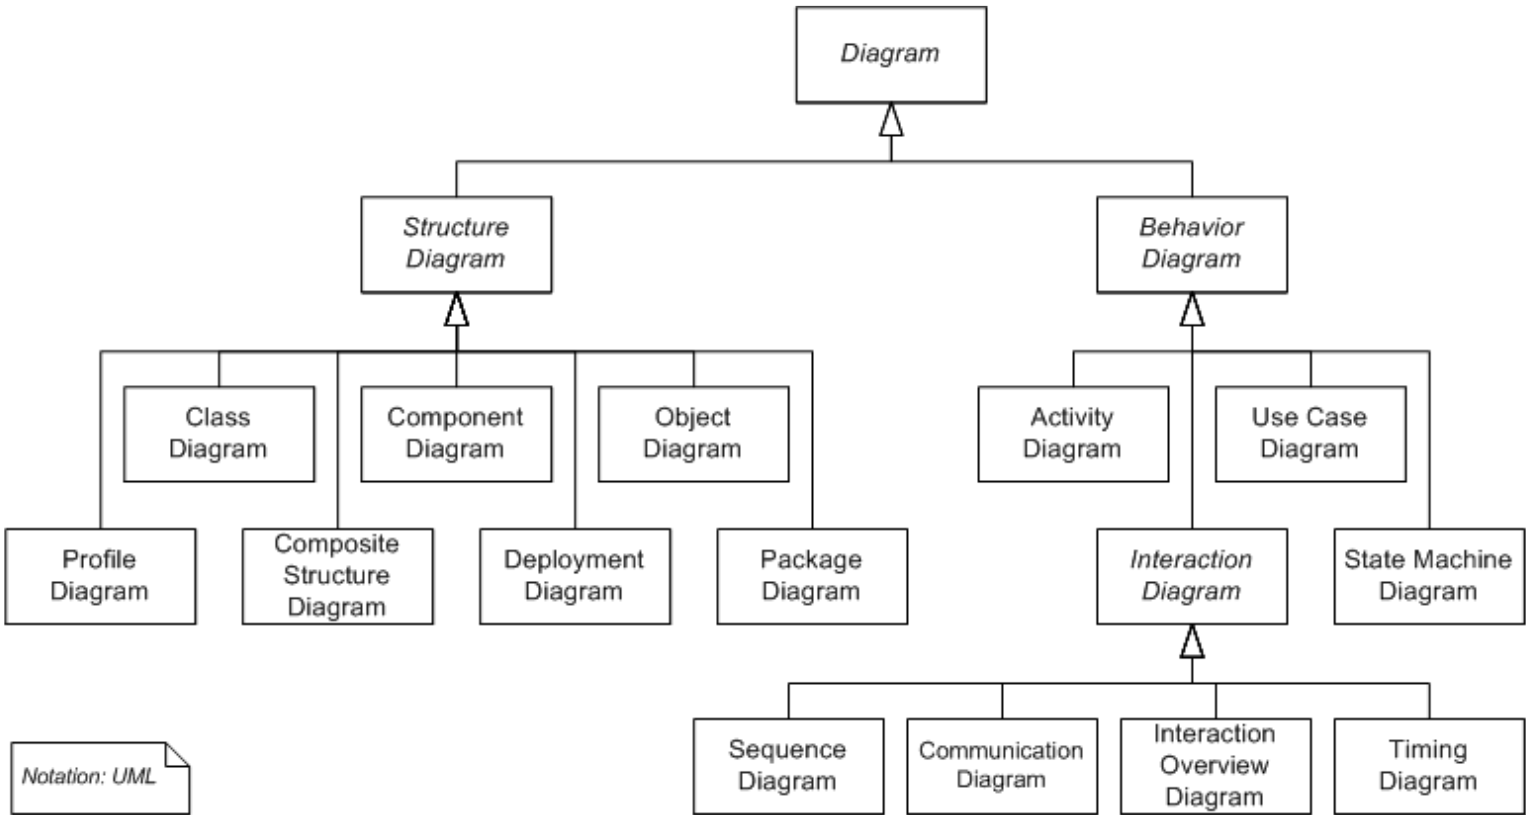
\includegraphics[width=\textwidth]{umlDiagrams.png}
\end{center}

Сама картинка --- это диаграмма классов UML, кстати.

Диаграммы делятся на две крупные категории --- структурные и поведенческие. Структурные диаграммы показывают структуру системы времени компиляции --- это прежде всего диаграмма классов, диаграмма компонентов, диаграмма пакетов и другие. Поведенческие диаграммы показывают, как система себя ведёт во время работы --- это диаграммы состояний, диаграммы последовательностей, диаграммы активностей, сюда же относят диаграммы случаев использования и другие, более специализированные диаграммы. Про почти все эти диаграммы будет подробно далее.

\subsubsection{Диаграмма классов, общий синтаксис}

Самая известная диаграмма UML --- это, пожалуй, диаграмма классов. Её внешний вид и описание элементов из книжки М. Фаулера ``UML. Основы'' (кстати, книга очень рекомендуется как быстрая справка по UML, информации в которой вполне достаточно, чтобы успешно пользоваться языком):

\begin{center}
	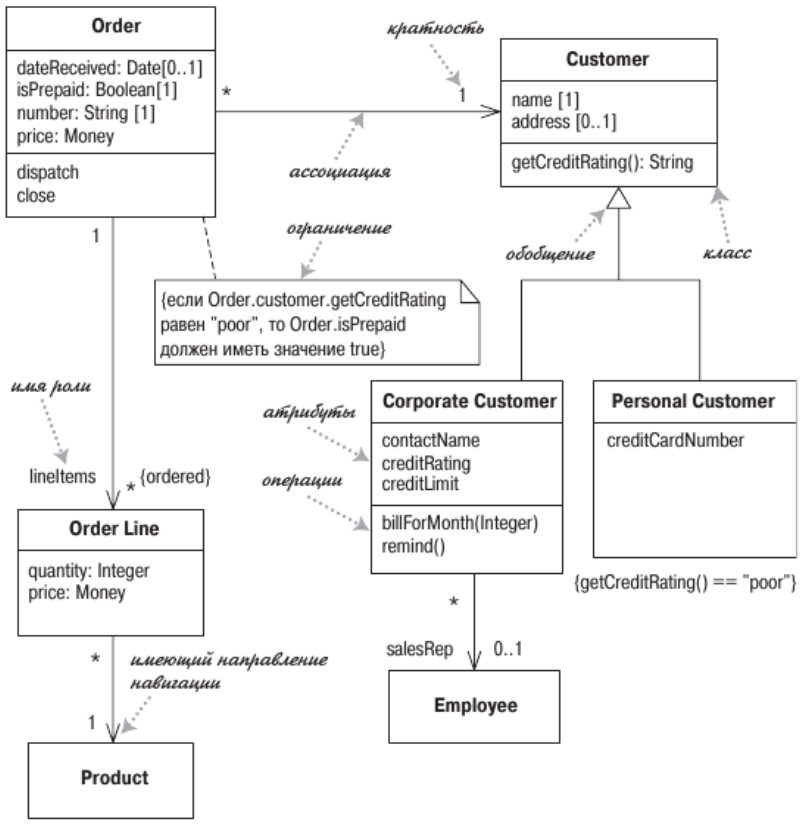
\includegraphics[width=0.8\textwidth]{umlClassDiagram.png}
	\attribution{М. Фаулер. ``UML. Основы''}
\end{center}

В общем-то, пояснений картинка не требует, надо только обратить внимание, что наследование в UML называется ``обобщение'' (generalization) и стрелка указывает на предка, а не на потомка (с этим часто путаются). Кратность ассоциации тоже может вызвать путаницу, она пишется у того конца ассоциации, к которому относится кратность. Например, Customer может иметь много Order (звёздочка означает ``0 или больше''), но у каждого Order ровно один Customer. 

Ещё одна важная особенность всех UML-диаграмм --- это то, что они допускают не отображать некоторую информацию, если автор считает её не важной в данном контексте (вспомните про точку зрения моделирования). Например, на рисунке выше неверно, что класс Employee не имеет ни методов, ни полей, просто автор посчитал, что они не важны и решил не загромождать диаграмму. То же касается и ассоциаций --- отсутствие множественностей или стрелок означает лишь, что они не специфицированы, они вполне могут быть выбраны самостоятельно программистом, который реализует систему.

\subsubsection{Атрибуты}

У диаграмм классов есть важная синтаксическая особенность --- атрибуты и ассоциации представляют собой с точки зрения синтаксиса языка одно и то же, просто отображаются по-разному. Например, диаграммы

\begin{center}
	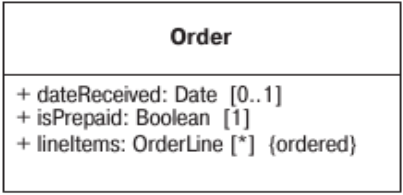
\includegraphics[width=0.3\textwidth]{attributes.png}
\end{center}

и

\begin{center}
	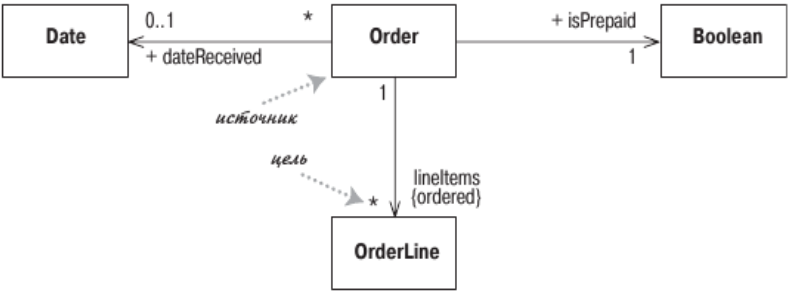
\includegraphics[width=0.7\textwidth]{associations.png}
\end{center}

означают в точности одно и то же. Атрибуты обычно используются, когда связи между классами не важны: когда типы атрибутов --- элементарные типы или перечисления (или даже структуры, короче, являются типами-значениями по смыслу; либо типы атрибутов --- это полноценные классы, но из третьесторонних библиотек). Ассоциации --- когда связи между классами важны для понимания архитектуры (чаще всего, когда типы атрибутов --- классы из реализуемой системы).

Ассоциациям самим разрешается иметь атрибуты (хотя в реальных диаграммах это встречается довольно редко), рисуется это вот так:

\begin{center}
	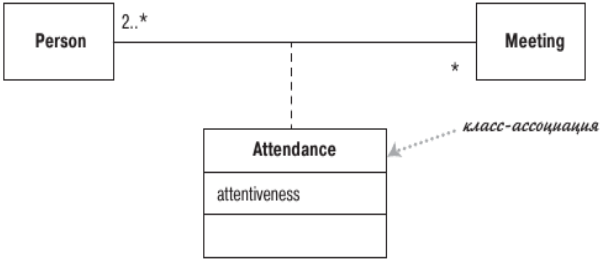
\includegraphics[width=0.65\textwidth]{classAssociation.png}
\end{center}

(все рисунки, как обычно, из книги М. Фаулера, ``UML. Основы.'')

Описание свойства внутри класса имеет в самом общем виде форму ``\verb|видимость имя: тип кратность = значение по умолчанию \{строка свойств\}|''. При этом видимость бывает \texttt{$+$ (public), $-$ (private), \# (protected), \textasciitilde (package)}. А кратность --- \texttt{1} (ровно 1 объект), \texttt{0..1} (ни одного или один), \texttt{*} (сколько угодно), \texttt{1..*}, \texttt{2..*}.

\subsubsection{Атрибуты и код}

Как диаграммы классов связаны с кодом лучше всего пояснить на примере. Если у нас есть такая диаграмма классов:

\begin{center}
	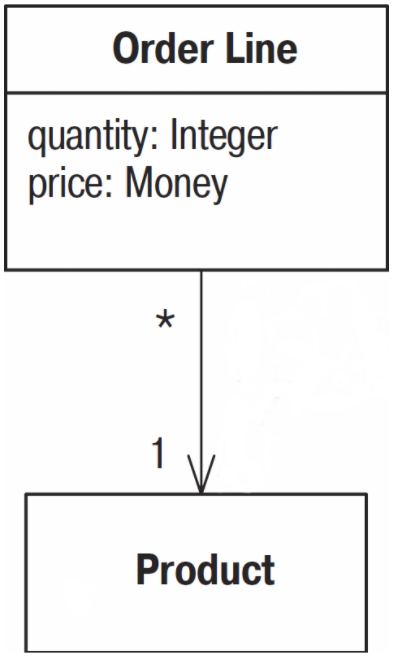
\includegraphics[width=0.2\textwidth]{orderLine.png}
\end{center}

то по ней можно написать (или сгенерировать, по крайней мере большую часть) вот такой код (для примера, на Java):

\begin{minted}{java}
public class OrderLine {
    private int quantity;
    private Product product;

    public int getQuantity() {
        return quantity;
    }

    public void setQuantity(int quantity) {
        this.quantity = quantity;
    }

    public Money getPrice() {
        return product.getPrice().multiply(quantity);
    }
}
\end{minted}

Класс Product тут для краткости не показан, благо на диаграмме про него всё равно никаких подробностей не приводится. Обратите внимание, что навигабельная ассоциация стала полем, а поле price в ходе реализации превратилось не в поле, а в вычислимое свойство. Такие преобразования тоже вполне допустимы, если программист-реализатор считает, что так удобнее.

С двунаправленными ассоциациями несколько хитрее, потому что при реализации требуется ещё некий механизм поддержания целостности обоих концов ассоциации. Например, диаграмма

\begin{center}
	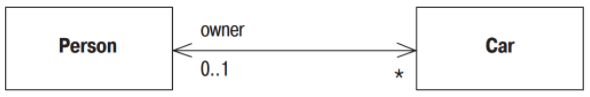
\includegraphics[width=0.5\textwidth]{twoWayAssociations.png}
\end{center}

могла бы быть реализована следующим образом (теперь на C\#, для разнообразия):

\begin{minted}{csharp}
class Car {
    public Person Owner {
        get { return _owner; }
        set {
            if (_owner != null) 
            {
                _owner.friendCars().Remove(this);
            }

            _owner = value;
            if (_owner != null) 
            {
                _owner.friendCars().Add(this);
            }
        }
    }
    private Person _owner;
}

class Person {
    public IList Cars {
        get { return ArrayList.ReadOnly(_cars); }
    }

    public void AddCar(Car arg) {
        arg.Owner = this;
    }

    private IList _cars = new ArrayList();

    internal IList friendCars() {
        // должен быть использован только Car.Owner
        return _cars;
    }
}
\end{minted}

В C\# нет аналога ключевому слову friend из C++, так что приходится использовать метод с пакетной видимостью, чтобы ограничить его использование. Но общий смысл тут такой, что при изменении одного конца ассоциации надо не забыть поменять и объект на другом конце --- сказать ему, что мы что-то добавили или что-то удалили.

\subsubsection{Интерфейсы}

На диаграмме классов есть целых два способа изображать интерфейсы: 

\begin{center}
	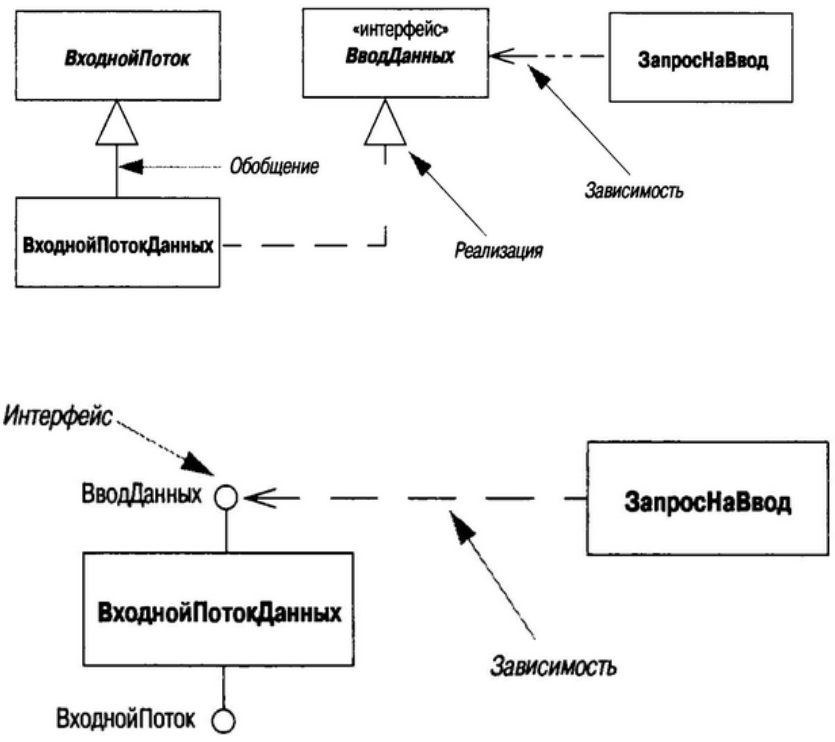
\includegraphics[width=0.6\textwidth]{interfaces.png}
	\attribution{М. Фаулер. ``UML. Основы''}
\end{center}

Так же, как в Java, реализация интерфейса и наследование от класса в UML суть разные вещи, реализация интерфейса рисуется пунктирной линией. Либо используется ``леденцовая'' нотация, когда реализуемый классом интерфейс рисуется как кружок с названием интерфейса, соединённый с классом линией. Такая нотация предпочтительней, если нам не очень важны методы интерфейса либо если интерфейсов много. Нотация со словом \verb|<<интерфейс>>| (или \verb|<<nterface>>| по-английски) используется, когда надо показат и методы интерфейса тоже (и тогда они пишутся как методы класса). Кстати, слова в ``ёлочках'' называются в UML \textit{стереотипами} и используются очень часто в самом языке и в механизме расширений через профили, когда придумывать новую фигуру для новой сущности не хочется (например, интерфейс --- это почти класс, так что он рисуется как класс, просто над ним пишется, что он интерфейс).

\subsubsection{Зависимости}

Потребление интерфейса рисуется как зависимость, пунктирной стрелкой. Зависимость --- наиболее общий вид связи между классами, она означает просто, что один класс (или интерфейс) что-то знает про другой (например, он ему нужен, чтобы скомпилироваться). Зависимости могут быть уточнены стереотипами, некоторые из которых прописаны в стандарте:

\begin{itemize}
	\item call --- один класс вызывает метод другого;
	\item create --- один класс создаёт в каком-то из свих методов объект другого;
	\item derive --- 
	\item permit 
	\item realize --- один класс реализует другой (например, абстрактный класс);
	\item substitute
	\item instantiate
	\item refine --- один класс является уточнением другого (что бы ни понимал под этим архитектор);
	\item use --- один класс использует другой в своей реализации;
	\item trace --- зависимость, которая может быть установлена даже между элементами с разных диаграмм, означает, что один элемент как-то влияет на другой --- например, случай использования может быть связан отношением trace с классами, которые его реализуют.
\end{itemize}

Рисуются зависимости вот так:

\begin{center}
	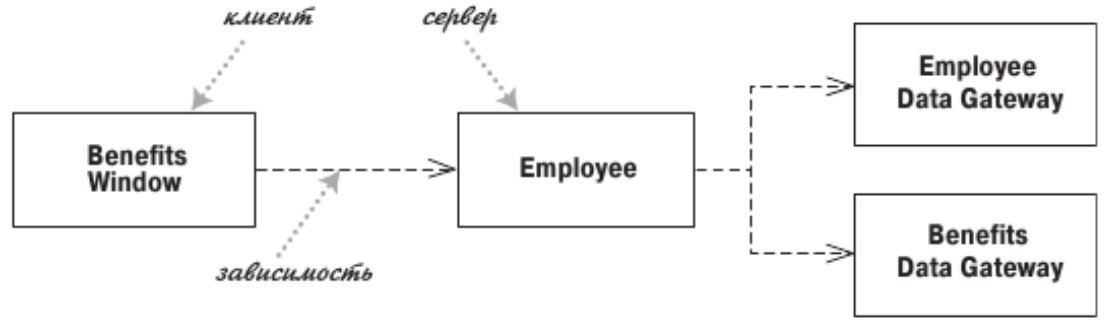
\includegraphics[width=0.7\textwidth]{dependencies.png}
	\attribution{М. Фаулер. ``UML. Основы''}
\end{center}

Если надо уточнить зависимость, то уточняющее слово (call, create и т.д.) пишется в ``ёлочках'' над линией по центру.

\subsubsection{Агрегация и композиция}

Агрегация и композиция ---- дальнейшие уточнения ассоциации. На самом деле, если на диаграмме нарисована просто ассоциация, то при реализации мы вправе выбрать, агрегацию или композицию использовать. Разница между агрегацией и композицией --- во владении объектами, которые участвуют в ассоциации. Агрегация не предполагает владения:

\begin{center}
	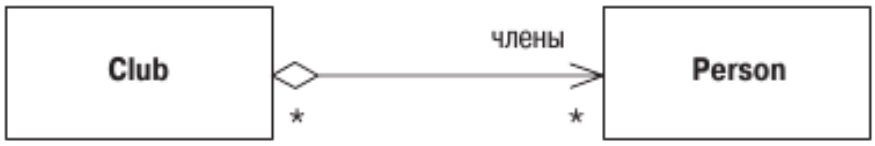
\includegraphics[width=0.5\textwidth]{aggregation.png}
\end{center}

Человек и клуб могут существовать независимо друг от друга, и когда закрывается клуб, его члены продолжают существовать (если это не тоталитарная секта). На диаграмме выше нарисовано, что в клубе может состоять несколько человек, и человек может состоять в нескольких клубах, при этом клуб знает о человеке, но не владеет им.

Композиция говорит, что один объект владеет другим объектом, то есть время их жизни связано и ``хозяин'' отвечает за удаление подчинённого ему объекта. Например, если мы пишем графический редактор, вполне может быть, что мы сделаем так:

\begin{center}
	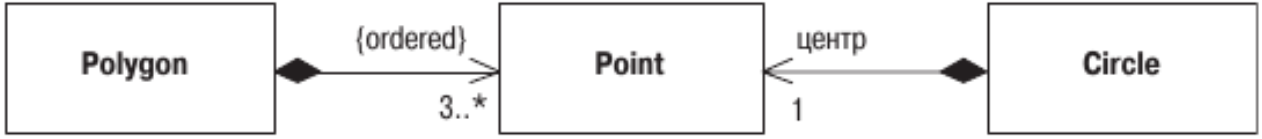
\includegraphics[width=0.7\textwidth]{composition.png}
\end{center}

Здесь многоугольник состоит из точек, и когда мы удаляем многоугольник, удаляются и все точки, которые его определяют. Круг тоже имеет одну точку --- центр круга, и тоже, удаляем круг --- удаляется и его центр. Так что и круг и многоугольник владеют своими точками, но у каждой точки вов ремя исполнения может быть только один хозяин.

Агрегация и композиция важны, если в итоге мы будем писать на C++, там они помогают следить за тем, кто в итоге должен освободить память из-под объекта. Для языков со сборкой мусора это не так важно (хотя и полезно знать, кто кем владеет), поэтому агрегация с композицией используются в диаграммах классов довольно редко --- обычно архитекторы ограничиваются ассоциациями, не специфицируя, агрегация эта конкретная ассоциация или композиция.

С точки зрения нотации надо запомнить, что агрегация --- более слабое отношение, чем композиция, поэтому и ромбик в случае агрегации не закрашен. И ромбики рисуются около контейнера (то есть клуб содержит людей, а не наоборот) --- можно понимать ромбик как оперение стрелы, указвающей от контейнера к содержащемуся в нём объекту. Ещё один небольшой пример:

\begin{center}
	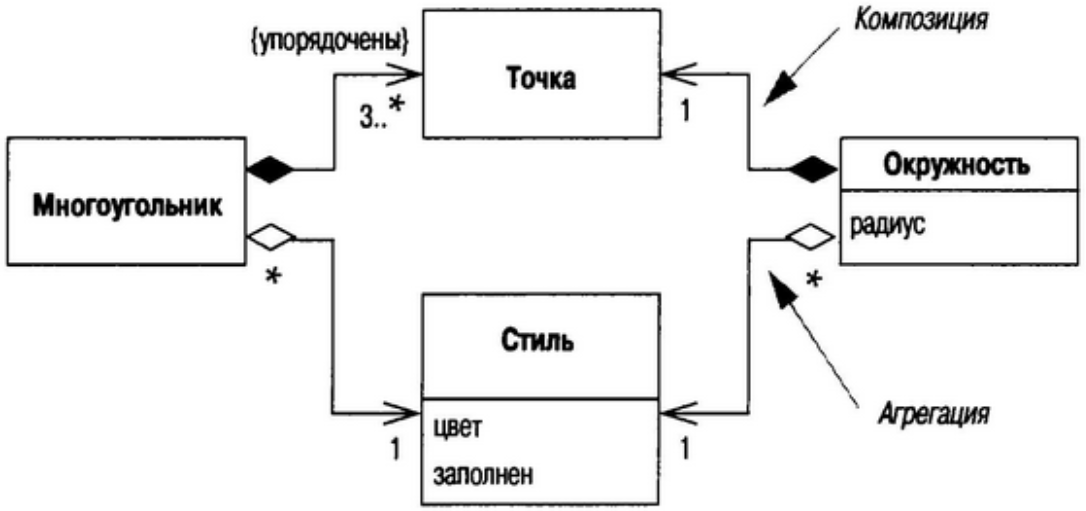
\includegraphics[width=0.6\textwidth]{aggregationAndCompositionExample.png}
	\attribution{М. Фаулер. ``UML. Основы''}
\end{center}

Многоугольник и окружность владеют своими точками, но не владеют стилями --- у каждой геометрической фигуры должен быть стиль, но стили существуют независимо и могут переиспользоваться между фигурами. Точки между фигурами переиспользованы быть не могут.

\subsubsection{Шаблоны и перечисления}

В отличие от первых версий Java, в UML синтааксис для шаблонных классов (или генериков) был всегда: параметры-типы перечисляются через запятую в пунктирном прямоугольнике в правом верхнем углу класса. Инстанцирование шаблона (то есть подстановка фактических параметров-типов вместо формальных) рисуется либо как просто класс, у которого указано, что куда подставляется, либо как наследование со стереотипом \verb|<<bind>>|, как на рисунке ниже:

\begin{center}
	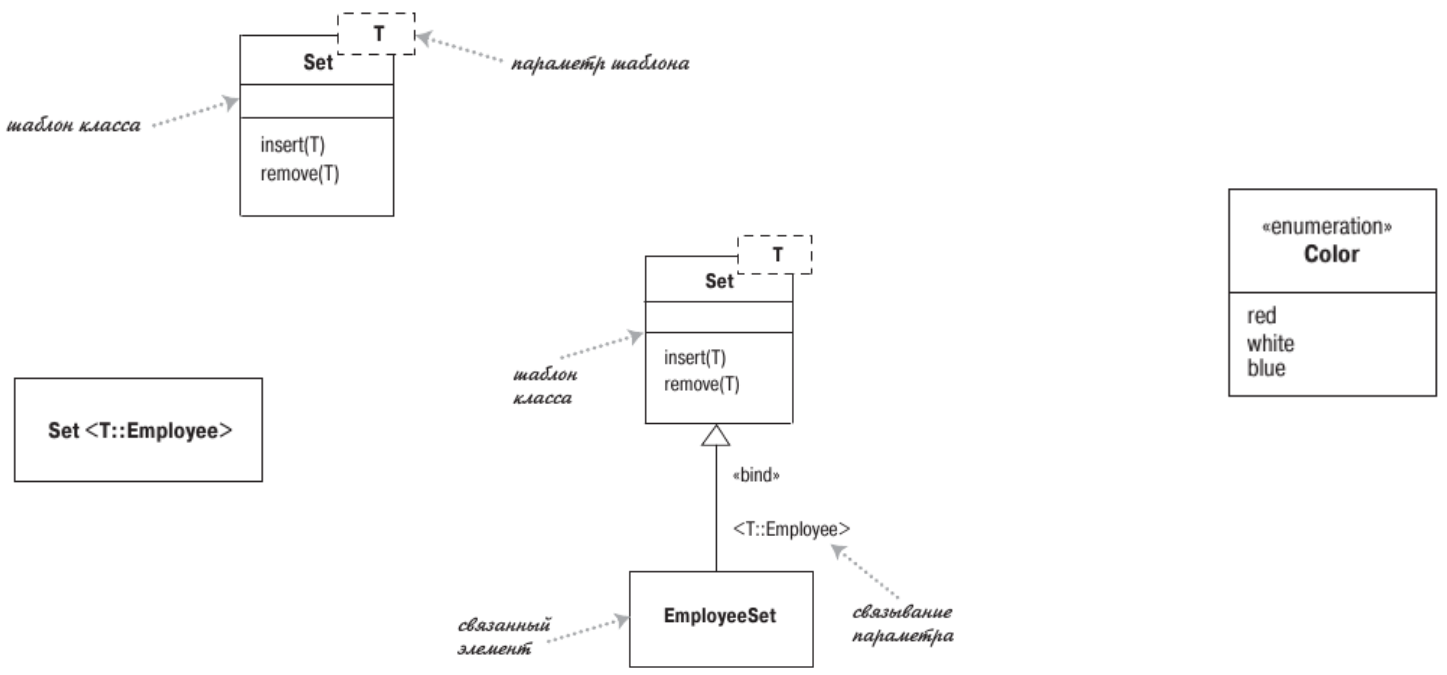
\includegraphics[width=\textwidth]{genericsAndEnums.png}
	\attribution{М. Фаулер. ``UML. Основы''}
\end{center}

Второй способ используется, когда экземпляр шаблона доопределяет ещё какие-нибудь методы и поля (например, классы QList<T> и QStringList в библиотеке Qt, второй является специализацией первого для типа QString, но добавляет ещё специфичные методы, например, join()).

На рисунке также видно, как задаются перечисления. Используется стереотип \verb|<<enumeration>>| и просто перечисляются элементы.

\subsection{Диаграммы пакетов}

Следующий вид диаграмм UML --- диаграммы пакетов. Это тоже структурные диаграммы, нужны они для того, чтобы показать разбиение кода по пакетам, либо сгруппирвоать по пакетам саму модель. ``Пакет'' в UML означает более-менее то же, что пакет в Java или пространоство имён в C++. Синтаксис диаграммы пакетов очень простой:

\begin{center}
	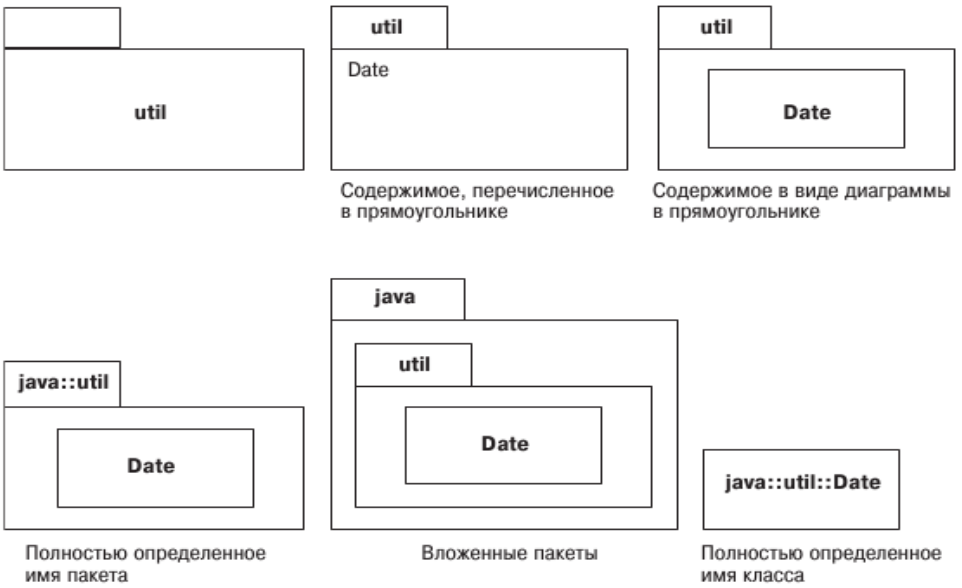
\includegraphics[width=0.8\textwidth]{packageDiagrams.png}
	\attribution{М. Фаулер. ``UML. Основы''}
\end{center}

На диаграммах пакетов также могут рисоваться компоненты и классы, которые в этих пакетах находятся. Это ещё одна не вполне очевидная особенность UML --- диаграммы не являются отдельными языками, более того, в спецификации UML разбиения на диаграммы нет. Язык описывается единой метамоделью (сгруппированной по пакетам, кстати), а какие элементы на каких диаграммах рекомендуется рисовать, описано только в приложении к стандарту. Так что теоретически всё что угодно можно рисовать где угодно, хотя правила здравого смысла иногда этому мешают. Например, рисовать сущности структурных и поведенческих диаграмм на одной диаграмме нельзя, потому что это может сильно запутать читателя.

Диаграммы пакетов полезны ещё тем, что на них можно визуализировать зависимости между пакетами:

\begin{center}
	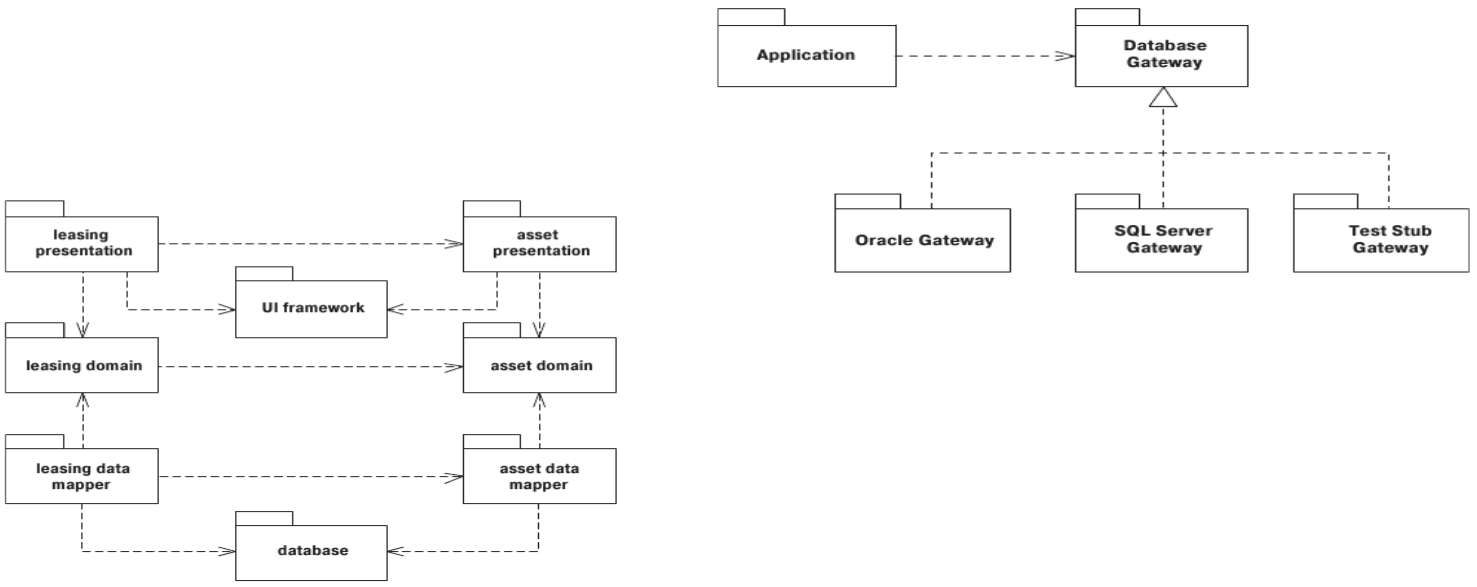
\includegraphics[width=0.95\textwidth]{packageDependencies.png}
	\attribution{М. Фаулер. ``UML. Основы''}
\end{center}

Просто зависимость означает, что пакет как-то связан с другим пакетом (так же, как зависимость между классами), стрелка ``реализация'' означает, что в пакете-предке есть хотя бы один класс, являющийся предком хотя бы одного класса из пакета-потомка, либо интерфейс, который пакет-потомок реализует. На самом деле, часто отношение реализации рисуют в том случае, если смысл пакета-предка в архитектуре --- содержать интерфейсы или абстрактные классы, которые должны реализовывать другие пакеты.

\subsection{Диаграммы объектов}

Диаграммы объектов визуализируют объекты в памяти во время работы программы и отношения между ними (так что по смыслу относятся к поведенческим диаграммам, но все их всё равно считают структурными, поскольку они описывают структуру времени выполнения, а не характер взаимодействия объектов). Диаграммы объектов можно понимать как снимок в какой-то определённый момент времени состояния системы, при этом множество всех возможных состояний описывается диаграммой классов.

Диаграммы объектов используют в двух случаях:

\begin{itemize}
	\item чтобы визуализировать и проиллюстрировать диаграммы классов (как на рисунке ниже, по диаграмме классов не сразу очевидно, что она описывает дерево, а по диаграмме объектов --- сразу);
	\item чтобы разобраться во взаимосвязях реально существующих объектов предметной области, ещё до того, как создана первая диаграмма классов (и тогда диаграмма классов будет на самом деле наведением классификации на объекты, выделенные на диаграмме объектов). Обращаю внимание на этот случай использования, мы увидим примеры применения диаграмм объектов в качестве инструмента анализа предметной области, когда дойдём до методологии предметно-ориентированного проектирования.
\end{itemize}

Синтаксис диаграмм объектов показан на этом рисунке:

\begin{center}
	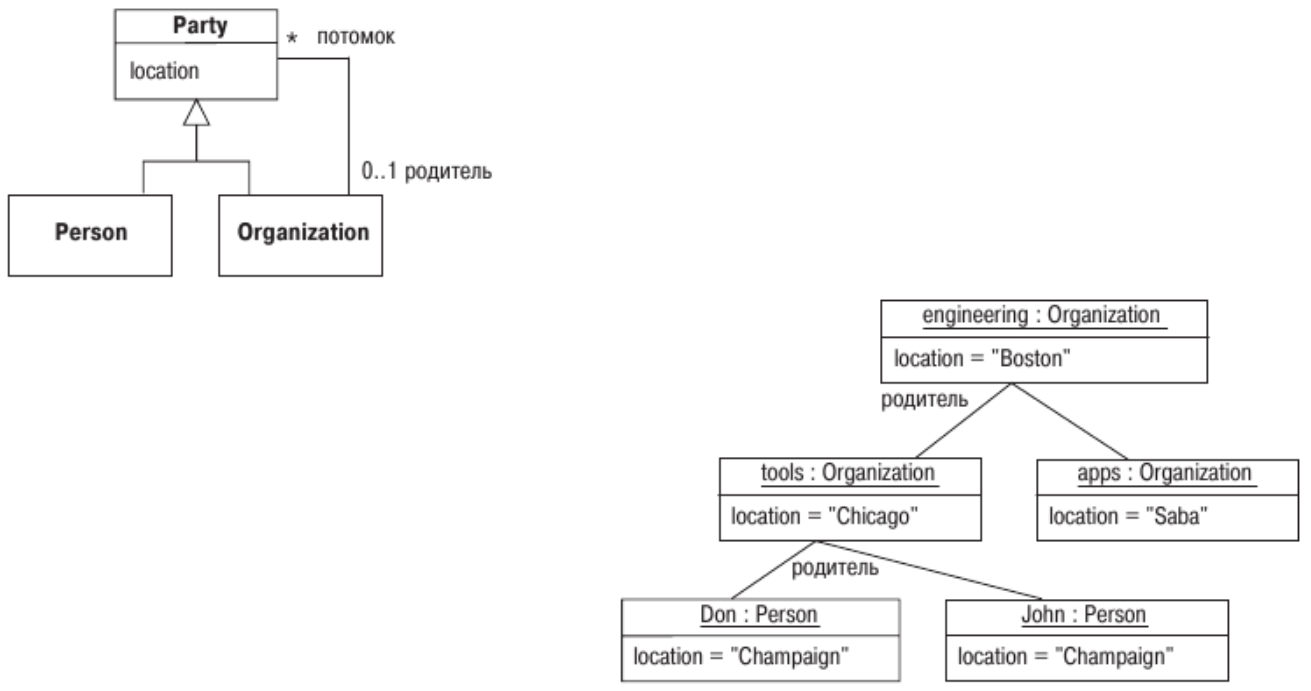
\includegraphics[width=0.9\textwidth]{objectDiagrams.png}
	\attribution{М. Фаулер. ``UML. Основы''}
\end{center}

Объект рисуется как класс, только его имя подчёркивается, указываается его тип, и каждому атрибуту ставится в соответствие значение.

\subsection{Диаграммы компонентов}

Диаграммы компонентов --- пожалуй, самые полезные для архитектора диаграммы UML. На них изображаются компоненты, из которых состоит система или подсистема, и взаимосвязи между ними. Точного определения термина ``компонент'' не существует, но все интуитивно представляют, что это такое --- нечто структурно связанное и больше, чем класс. Компонентами могут быть пакеты, пространства имён, сборки, .dll/.so-файлы, отдельные веб-сервисы в распределённом приложении и т.д. В общем, это именно то, из чего состоит высокоуровневая архитектура приложения.

Почему диаграммы компонентов важнее и полезнее диаграмм классов --- они переживают большую часть рефакторингов. Диаграммы классов придётся перерисовывать каждый раз, когда кто-то поменял название какого-нибудь класса или даже метода, добавил поле и т.д. Диаграммы компонентов неизменны до глобальной переработки архитектуры, которая в типичных проектах происходит только раз в несколько лет, так что у диаграмм компонентов много шансов сохранить свою актуальность в долгосрочной перспективе.

Полезны диаграммы компонентов как вид ``с высоты птичьего полёта'' на создаваемую систему. Например, вот диаграмма, описывающая высокоуровневую архитектуру проекта QReal (\url{https://github.com/qreal/qreal}, инструмент для создания визуальных предметно-ориентированных языков и работы с ними):

\begin{center}
	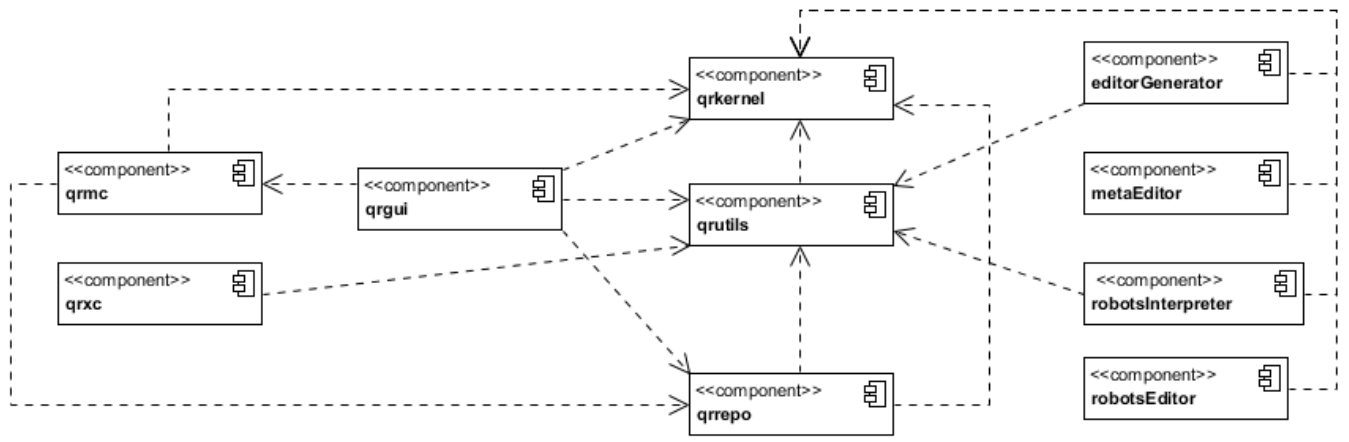
\includegraphics[width=0.95\textwidth]{componentDiagrams.png}
\end{center}

Связи между компонентами тут означают зависимости по сборке, каждый компонент --- это отдельный проект, который собирается в отдельный .dll/.so-файл. По такой диаграмме можно очень быстро рассказать общую архитектуру проекта: qrkernel ни от кого не зависит, там находятся классы, общие для всей системы; qrutils содержит полезную функциональность, используемую в других модулях; qrrepo --- репозиторий, где хранятся данные, с которыми QReal работает; qrgui --- пользовательский интерфейс; qrmc и qrxc --- это компиляторы визуальных языков, с которыми работает Real; editorGenerator, metaEditor, robotsInterpreter, robotsEditor --- это плагины инструментальной поддержки работы с визуальными языками. Конечно, это не полноценное архитектурное описание, но даже этого достаточно, чтобы было понятно, куда смотреть в исходниках.

Вот описание синтаксиста диаграмм компонент, на сей раз с сайта \url{http://www.uml-diagrams.org} (очень рекомендую, как быструю справку по синтаксису и как набор примеров с пояснениями):

\begin{center}
	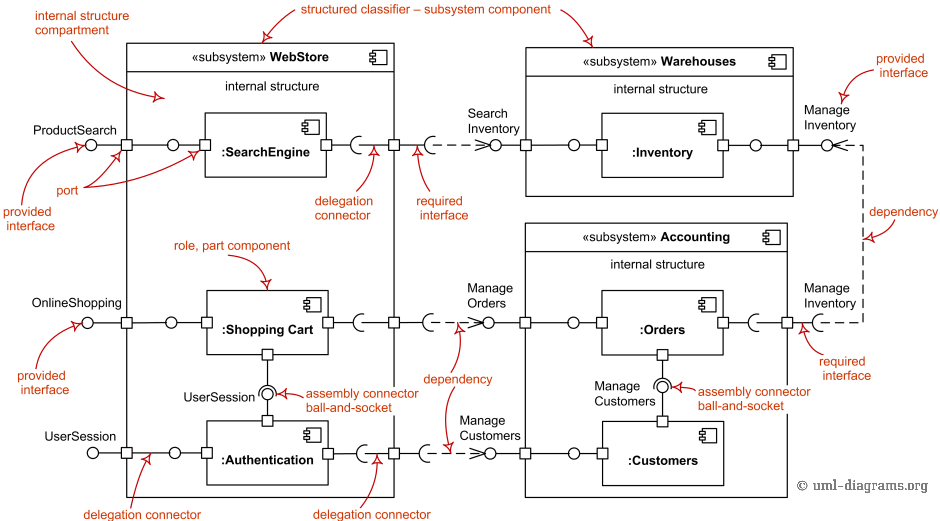
\includegraphics[width=0.95\textwidth]{componentDiagramsOverview.png}
	\attribution{\url{http://www.uml-diagrams.org}}
\end{center}

Видно, что компоненты могут быть вложенными друг в друга, что они могут иметь интерфейсы (так же, как и классы, но на диаграммах компонентов чаще всего используется только ``леденцовая'' нотация). У компонентов есть порты, кторые могут предоставлять или потреблять интерфейсы, но порты часто не рисуются, а подразумеваются, поскольку обычно порт имеет только один интерфейс. Порты бывают полезны для изображения делегирования --- что компонент просто перенаправляет запросы вложенному компоненту. Слова \verb|<<subsystem>>| и ``internal structure'' опциональны (и обычно не пишутся).

\end{document}
